% Fig. 1: task-oriented pipeline (training proxy == evaluation truth)
% Compile: xelatex pipeline.tex  (preview: pdftoppm -png -r 120 pipeline.pdf x)
% Page auto-fits the picture (standalone.cls not available in BasicTeX).
\documentclass[12pt]{article}
\usepackage{amsmath,amssymb}
\usepackage{tikz}
\usetikzlibrary{positioning,arrows.meta,calc}
\pagestyle{empty}
\setlength{\topmargin}{-1in}
\setlength{\headheight}{0pt}
\setlength{\headsep}{0pt}
\setlength{\oddsidemargin}{-1in}
\setlength{\parindent}{0pt}

\definecolor{evalblue}{RGB}{213,229,245}
\definecolor{trainorange}{RGB}{252,229,205}
\definecolor{sharedgreen}{RGB}{217,234,211}
\definecolor{modelgrey}{RGB}{235,235,235}

\begin{document}
\setbox0=\hbox{%
\scriptsize
\begin{tikzpicture}[
  box/.style={draw, rounded corners=2pt, align=center, inner sep=4.5pt},
  lbl/.style={font=\tiny\itshape},
  arr/.style={-{Stealth[length=2.5mm]}, semithick},
  oarr/.style={-{Stealth[length=2mm]}, dashed, gray},
]

% ---- row 1: mixture -> separator -> shared front-end ----
\node[box, fill=modelgrey] (mix) at (0,0)
  {Mixture\\[1pt] $y(t)=\sum_{k=1}^{K} w_k s_k(t)+n(t)$\\[1pt]
   $K\in\{1,2,3\}$, $\mathrm{SIR}\approx 0$\,dB};

\node[box, fill=modelgrey, right=0.6cm of mix, align=center] (sep)
  {Slot separator\\ (complex CNN)\\[1pt]
   $K_{\max}{=}4$ mask slots\\ $+$ occupancy / count heads};

\node[box, fill=sharedgreen, right=1.5cm of sep, align=left, inner sep=6pt]
  (fe) {\textbf{Compensated receiver front-end}\\
  shared implementation: training \& evaluation\\[2pt]
  1.\ oracle down-conversion $e^{-j2\pi f_k t/f_s}$\\
  2.\ RRC matched filter\\
  3.\ symbol-grid sampling $0{:}{:}16$\\
  4.\ unit-power normalisation\\
  5.\ phase alignment $\rho$ (fit detached)};

% ---- oracle side information, above the sep--fe gap ----
\node[box, dashed, inner sep=4pt, align=center] (oracle)
  at ($(sep.north)!0.5!(fe.north) + (0,1.2)$)
  {Generator side information (oracle):\\
   true sources $s_k$, carriers $f_k$, modulations $m_k$};

% ---- column under the front-end: eval (top), train (bottom) ----
\node[box, fill=evalblue, below=0.9cm of fe, align=center, inner sep=5pt]
  (eval)
  {hard minimum-distance decisions\\[1pt]
   \textbf{compensated SER $+$ Gray BER}\; (evaluation truth)};

\node[box, fill=trainorange, below=0.45cm of eval, align=center,
      inner sep=5pt] (train)
  {soft logits $\ell_n(c)=-|\hat{z}_n-c|^2/\sigma^2$,
   masked softmax CE\\[1pt]
   \textbf{$\mathcal{L}_{\mathrm{soft\text{-}SER}}$}\; (training proxy)};

% ---- arrows ----
\draw[arr] (mix) -- (sep);
\draw[arr] (sep) -- node[lbl, align=center, below=0pt]{PIT $\pi^*$\\
  $(\hat{s}_{\pi(k)}, s_k)$} (fe);
\draw[arr] (fe.south) -- (eval.north);
\draw[arr] (eval.south) -- (train.north);
\draw[oarr] (oracle.south) ++(-1.4,0) --
  node[lbl, pos=0.4, left]{$s_k, m_k$ (labels)}
  ($(sep.east)!0.5!(fe.west) + (0,0.35)$);
\draw[oarr] (oracle.south) ++( 1.4,0) --
  node[lbl, pos=0.5, right]{$f_k$} (fe.north);

% waveform PIT loss, lower-left (also fills the empty corner)
\node[box, fill=modelgrey, align=center] (wloss)
  at ($(mix.south) + (1.1,-2.6)$)
  {waveform PIT loss\\[1pt]
   $-\,\Delta$SI-SDR ($+$ MSE anchor)};
\draw[arr] (wloss.north) -- ($(sep.south)+(-0.9,0)$);

% gradients: train -> left -> down -> along the bottom -> up into the separator
\draw[arr, trainorange!60!black, dashed]
  (train.west) -- ++(-0.9,0) -- ++(0,-1.1)
  -| node[lbl, pos=0.25, below]{gradients}
  ($(sep.south)+(0.9,0)$);

\end{tikzpicture}}%
\pdfpagewidth=\dimexpr\wd0+6pt\relax
\pdfpageheight=\dimexpr\ht0+\dp0+6pt\relax
\hoffset=3pt
\voffset=3pt
\leavevmode\usebox0
\end{document}
